\documentclass[11pt]{article}
\usepackage[final]{acl}
\usepackage{times}
\usepackage{latexsym}
\usepackage[T1]{fontenc}
\usepackage[utf8]{inputenc}
\usepackage{microtype}
\usepackage{inconsolata}
\usepackage{graphicx}
\usepackage{booktabs}
\usepackage{amsmath}
\usepackage{amssymb}
\usepackage{multirow}
\usepackage{balance}
\usepackage{float}
\makeatletter
\setlength{\@dblfptop}{0pt}
\makeatother

\title{Translation Is Not Representation:\\English-Hub Routing in Cross-Lingual Bias Benchmarks}

\author{Hak Hyun Kim \\
  Dartmouth College \\
  \texttt{hak.hyun.kim.gr@dartmouth.edu} \\\And
  Benjamin Huh \\
  Dartmouth College \\
  \texttt{benjamin.j.huh.24@dartmouth.edu}}

\begin{document}
\maketitle

\begin{abstract}
Cross-lingual bias benchmarks such as JBBQ and KoBBQ translate English bias probes and compare scores across languages, assuming the translated probe measures the same construct. We test this assumption at the representation and behavioral levels using 13B-parameter models matched on architecture but differing in language-training regime. A \textit{multi-anchor logit lens} shows that an English-centric model (Llama~2) processes Japanese and Korean inputs predominantly through English-script predictions in its middle layers, even where Centered Kernel Alignment (CKA) between languages is high: geometric convergence masks English-hub routing. Matched continual-adaptation comparisons show that target-language adaptation reduces this English-script mass: from $0.77$ to $0.56$ after Japanese adaptation (Swallow), and from $0.78$ to $0.71$ after Korean adaptation (koen), while balanced bilingual pretraining (LLM-jp) lowers it further to $0.19$. Behaviorally, every model is more stereotype-biased in English than in Japanese, with gaps from $0.13$ to $0.14$, but this asymmetry is language-specific: in Korean it is weak and disappears after Korean adaptation, with Korean nearly as stereotype-leaning as English. Yet patching English hub states into target-language processing does not transplant this bias. Cross-lingual bias scores thus reflect genuine language-specific behavior, not an English-pivot artifact, even though the underlying representations are not comparable. We distill this dissociation between representation and behavior into a four-step audit protocol for translated bias benchmarks.
\end{abstract}

% Section break
\section{Introduction}

Consider a BBQ age item in which an older visitor and a college-age neighbor talk about their favorite drinks \citep{parrish-etal-2022-bbq}. When a 13B-parameter language model continues this prompt in English, it generates a neutral exchange about ice preferences. The same model, given the faithful Japanese translation from JBBQ \citep{yanaka-etal-2025-jbbq}, instead produces a culturally specific continuation centered on \textit{nihonshu} (Japanese rice wine). The translation preserves the event, yet the model activates entirely different cultural associations.

This example illustrates a broader problem. Cross-lingual bias benchmarks, including JBBQ, KoBBQ \citep{jin-etal-2024-kobbq}, and MBBQ \citep{neplenbroek-etal-2024-mbbq}, evaluate models by translating English bias probes and comparing scores across languages. The implicit assumption is that translation preserves the measurement construct: that the same question probes the same bias in both languages. This assumption, known as measurement invariance in psychometrics \citep{vandenberg2000review}, has not been tested at the representation level.

We investigate this assumption by examining what happens inside the model when it processes paired prompts in English and a translated language. We use four 13B-parameter models that share the Llama architecture but differ in language-training regime: an English-centric base (Llama~2), the same base continually pretrained on Japanese (Swallow) and on Korean (Llama-2-koen), and a from-scratch balanced bilingual model (LLM-jp). Because the Llama-2/Swallow and Llama-2/koen pairs are matched on architecture and initialization, they isolate much of the adaptation effect from scale and architecture, while retaining tokenizer extension as part of the adaptation regime. We probe all 41 transformer layers on 2,142 English/Japanese BBQ/JBBQ pairs and a Simply-Transferred English/Korean BBQ/KoBBQ subset, combining CKA, a binned Logit Lens, and a multi-anchor (script-mass) Logit Lens that measures English-hub routing directly. Our key findings are:

\begin{enumerate}
\item \textbf{Geometric convergence masks English-hub routing.} CKA between an English and a translated prompt can be high while a multi-anchor Logit Lens shows the model predicting predominantly English-script tokens in its middle layers. Matched continual-adaptation comparisons (Llama~2$\rightarrow$Swallow and Llama~2$\rightarrow$koen, identical initialization and architecture) show that target-language adaptation \textit{reduces} this hub mass ($0.77\rightarrow0.56$ in Japanese; $0.78\to0.71$ in Korean), and balanced bilingual training minimizes it ($0.19$). CKA does not reveal any of this: Swallow has the \textit{highest} CKA of all models yet still routes through English.

\item \textbf{The behavioral bias asymmetry is language-specific.} In Japanese, every model assigns from $0.13$ to $0.14$ more probability to the stereotyped answer in English than in Japanese (95\% CI excludes zero), with Japanese near chance. In Korean the asymmetry is weak ($+0.05$ for the base model) and vanishes after Korean adaptation, with Korean nearly as stereotype-leaning as English: English is not universally more biased.

\item \textbf{Hub routing does not transplant bias.} Injecting English hub-layer states into target-language processing (both at the CKA-peak layer and across the full hub band) leaves the target-language stereotype preference unchanged relative to a random-direction control, in every model and in both Japanese and Korean. The cross-lingual bias gap is therefore genuine language-specific behavior, not an English-pivot artifact, even though it is computed over representations that are not comparable.
\end{enumerate}

% Section break
\section{Related Work}

\paragraph{Cross-lingual bias benchmarks.}
BBQ \citep{parrish-etal-2022-bbq} provides bias probes across nine social categories. Its translations include JBBQ \citep{yanaka-etal-2025-jbbq}, KoBBQ \citep{jin-etal-2024-kobbq}, and MBBQ \citep{neplenbroek-etal-2024-mbbq}. Prior work compares aggregate bias scores across languages but does not examine whether the underlying representations are comparable. \citet{goldfarb-tarrant-etal-2021-intrinsic} show that intrinsic bias metrics do not correlate with application-level bias, raising questions about what representation-level measures actually predict. We extend this line of inquiry to the cross-lingual setting.

\paragraph{Cross-lingual representations.}
Multilingual models have been argued to develop language-agnostic representations in middle layers \citep{pires-etal-2019-multilingual, conneau-etal-2020-emerging, chi-etal-2020-finding, wu-dredze-2020-languages}. These findings typically rely on geometric similarity measures such as CKA \citep{kornblith2019similarity}, probing classifiers, or alignment methods \citep{cao-etal-2020-multilingual}. Further work has shown that language-specific and language-neutral components can be separated from pre-trained multilingual representations \citep{libovicky-etal-2020-language}. However, recent work shows that English-centric models may process non-English inputs through an internal English pivot \citep{wendler2024llamas}, suggesting that geometric alignment may not entail functional equivalence. We make this pivot quantitative with a multi-anchor (script-mass) lens and, using models that share an initialization, show that target-language adaptation reduces it beyond what architecture and scale alone would explain.

\paragraph{Mechanistic interpretability.}
The Logit Lens \citep{nostalgebraist2020logitlens} projects intermediate hidden states to the vocabulary space, revealing how predictions evolve across layers. The Tuned Lens \citep{belrose2023eliciting} extends this with learned probes. Activation patching \citep{meng2022locating, geiger2021causal} and causal mediation analysis \citep{vig-etal-2020-causal} provide tools for establishing causal links between internal representations and model behavior. We combine these tools to characterize cross-lingual convergence beyond geometric similarity.

% Section break
\section{Experimental Setup}

\subsection{Models}

We study four 13B-parameter decoder-only models that share the Llama architecture (40 transformer layers, hidden size 5120) but differ in language-training regime:

\begin{itemize}
\item \textbf{Llama-2-13B} \citep{touvron2023llama2} (``Llama~2''): pretrained from scratch on a predominantly English corpus ($\sim$90\% English). Our English-centric base and the shared anchor for both matched pairs.
\item \textbf{Swallow-13B} \citep{fujii2024swallow}: \textbf{Llama-2-13B continually pretrained} on $\sim$100B additional tokens at a roughly 9:1 Japanese:English ratio, with the tokenizer extended by 11{,}176 Japanese subwords (vocabulary 43{,}176). Because it starts from Llama~2's weights, the Llama-2/Swallow pair separates Japanese adaptation from architecture and scale, though tokenizer extension remains part of the adaptation regime.
\item \textbf{Llama-2-koen-13B} \citep{lee2023llama2koen} (``koen''): Llama-2-13B continually pretrained on Korean and English ($>$60B tokens, vocabulary 46{,}336). The Korean analogue of the Llama-2/Swallow pair, used for directional replication.
\item \textbf{LLM-jp-3-13B} \citep{llmjp2024} (``LLM-jp''): pretrained from scratch on 2.1T tokens balanced across Japanese ($\sim$48\%) and English ($\sim$45\%). Represents balanced bilingual training with no continual-adaptation step.
\end{itemize}

All models use base (non-instruct) variants in bfloat16 and have untied input/output embeddings (\S\ref{sec:metrics}). We deliberately exclude models whose tokenizer cannot represent both languages. Stockmark-13B, for example, is trained from scratch on Japanese only and fragments English into roughly 34$\times$ more tokens; it fails the tokenizer feasibility check (Step~1 of our protocol, \S\ref{sec:protocol}) and cannot support a meaningful cross-lingual comparison, so we treat it as a feasibility-boundary case rather than a study model.

\subsection{Data}

Our primary analysis uses BBQ/JBBQ paired templates over five shared bias categories (Age, Disability Status, Gender Identity, Physical Appearance, Sexual Orientation); four BBQ categories without JBBQ counterparts are excluded. We sample 2{,}142 pairs stratified by category, each an English context (BBQ) and its Japanese translation (JBBQ) with answer choices and stereotype metadata. For the Korean replication we use KoBBQ \citep{jin-etal-2024-kobbq}, restricted to its \textit{Simply-Transferred} subset, the templates KoBBQ retains as direct cultural translations of BBQ, which therefore have clean English counterparts (aligned by KoBBQ's \texttt{bbq\_id}\footnote{KoBBQ's \texttt{bbq\_id} indexes the original BBQ \texttt{question\_index}, not the KoBBQ template id; aligning on the latter would mis-pair items.}). This yields 261 sampled English/Korean context pairs across 87 templates in the five shared categories; we treat the Korean results as a directional replication rather than an equal-scale analysis.

\subsection{Metrics}\label{sec:metrics}

Our representation-level analyses (CKA, Logit Lens, and the multi-anchor lens below) use only the context paragraph of each item, processed separately in each language; for these we extract the final-token hidden state at every layer $\ell \in \{0, \ldots, 40\}$, giving two matrices per layer $H^{\text{src}}_\ell, H^{\text{tgt}}_\ell \in \mathbb{R}^{N \times d}$ over the $N$ paired items. Our behavioral analyses (bias asymmetry and hub patching) instead use the full item (context, question, and the three answer options) to read out the model's stereotype preference. We score each answer by summing its candidate-token log probabilities conditioned on the prompt, then define $P_{\text{ster}}$ as the softmax probability of the stereotyped option among the three answer scores; Appendix~\ref{app:implementation} gives the implementation details.

We treat measurement equivalence as requiring two levels of alignment. First, paired prompts should occupy similarly organized regions of representation space; we call this \textit{geometric convergence} and measure it with linear CKA. Second, those representations should imply similar predictions; we probe this \textit{functional} side with a binned Logit Lens (Jensen-Shannon divergence between the languages' semantic-bin distributions) and, more directly, with a multi-anchor lens that asks \emph{in which language} the model is predicting. Geometric convergence alone is insufficient: two prompts can occupy similar neighborhoods while implying different next-token semantics.

\paragraph{CKA.} Linear Centered Kernel Alignment \citep{kornblith2019similarity} between $H^{\text{src}}_\ell$ and $H^{\text{tgt}}_\ell$ at each layer, measuring geometric alignment of the two languages' representation spaces.

\paragraph{Binned Logit Lens JSD.} We project each layer's final-token hidden state through the LM head, map predicted tokens to fixed bilingual semantic-anchor bins, and take the Jensen-Shannon divergence \citep{lin1991divergence} between the two languages' bin distributions. All our models have \emph{untied} input/output embeddings, so raw Logit Lens projections should be read with caution \citep{belrose2023eliciting}; because this condition is uniform across models, cross-model comparisons remain fair, and we corroborate every lens-based claim with the lens-free patching experiment below.

\paragraph{Multi-anchor Logit Lens (English-hub routing).} The binned lens asks \emph{what} a layer predicts; the multi-anchor lens asks \emph{in which script}. We classify every vocabulary token by its dominant Unicode script (Latin, Kana, Han, Hangul, digit, other) and, at each layer, sum the predicted probability mass per script. On a non-English input, the Latin-script mass measures how strongly the model predicts English tokens, i.e., routes through an English hub \citep{wendler2024llamas}. Japanese Kanji share the Han block with Chinese, so we score Kana separately as the Japanese-specific signal.

\paragraph{Hub patching.} To test whether English-hub routing drives the target-language bias, we inject English hidden states into target-language processing \citep{meng2022locating}. For each item we run the English prompt and read its residual stream at a hub layer (the CKA-peak layer; or, in a stronger variant, all layers 10 to 25), then overwrite the final prompt position of the target-language forward pass with the English state. We score the stereotyped, anti-stereotyped, and unknown answer options and report the stereotyped minus anti-stereotyped log-probability gap, comparing paired-English injection against a random-English control drawn from a different item. We use 300 ambiguous items per model and summarize the per-item paired minus random difference with a 10{,}000-sample bootstrap.

% Section break
\section{Results}

\subsection{Input-Level Tokenization}

Table~\ref{tab:input_stats} shows that the models tokenize the same text very differently. The English-centric Llama~2 over-fragments the target language (1.9$\times$ more tokens for Japanese than English, and 3.0$\times$ more for Korean), whereas the continually adapted models (Swallow, koen) and the balanced LLM-jp, which extend or rebuild the tokenizer, reach near-parity. Tokenizer efficiency already tracks the language-training regime.

\begin{table}[t]
\centering\small
\begin{tabular}{llcc}
\toprule
\textbf{Model} & \textbf{Regime} & \textbf{Vocab} & \textbf{Tgt/EN} \\
\midrule
Llama-2 & EN-centric & 32{,}000 & 1.93 \\
Swallow & $+$JA continual & 43{,}176 & 1.10 \\
LLM-jp & balanced & 99{,}574 & 0.87 \\
\midrule
Llama-2 (KO) & EN-centric & 32{,}000 & 2.98 \\
koen & $+$KO continual & 46{,}336 & 0.88 \\
\bottomrule
\end{tabular}
\caption{Tokenizer statistics. Tgt/EN is the mean target-to-English token-count ratio over sampled contexts. The English-centric base over-fragments both Japanese and Korean; adapted and balanced models do not.}
\label{tab:input_stats}
\end{table}

\subsection{Geometric Convergence Masks English-Hub Routing}

\begin{figure*}[t]
  \centering
  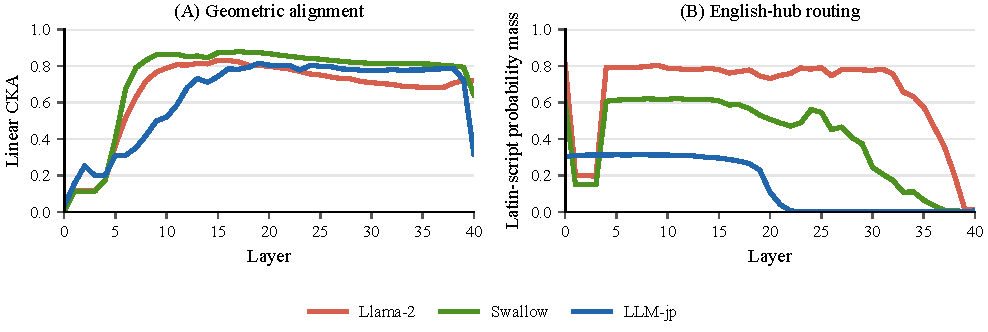
\includegraphics[width=\textwidth]{figures/fig_hub_routing.pdf}
  \caption{Geometric convergence masks English-hub routing (English/Japanese). (A) CKA between English and Japanese hidden states is high for all three models; the English-centric Llama~2 is no lower than the balanced LLM-jp. (B) Multi-anchor lens: the English-script (Latin) probability mass on \emph{Japanese} input stays near 0.78 through Llama~2's middle layers but is low for LLM-jp. High CKA coincides with heavy English routing.}
  \label{fig:hub}
\end{figure*}

\begin{figure}[tb]
  \centering
  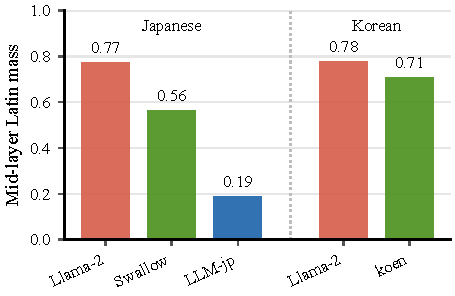
\includegraphics[width=.95\columnwidth]{figures/fig_adaptation.pdf}
  \caption{Mid-layer (layers 10 to 25) Latin mass on target-language input. Adaptation lowers English-hub routing; balanced bilingual training lowers it further.}
  \label{fig:adapt}
\end{figure}

Figure~\ref{fig:hub}A shows strong geometric convergence: CKA between English and Japanese hidden states peaks at 0.83 (Llama~2, layer 15), 0.88 (Swallow, layer 17), and 0.82 (LLM-jp, layer 19). By CKA alone, all three look like they place the two languages in a shared space, and the English-centric Llama~2 looks \emph{no worse} than the balanced LLM-jp.

The multi-anchor lens reveals what CKA hides (Figure~\ref{fig:hub}B). For Japanese input, Llama~2 predicts overwhelmingly English-script tokens through its middle layers (Latin-script mass stays near 0.78 from layer 0 to 30 and collapses only at the final layer), while LLM-jp predicts Japanese-script tokens from the start. Averaged over the hub band (layers 10 to 25), English-script mass is 0.77 for Llama~2, 0.56 for Swallow, and 0.19 for LLM-jp. Geometric convergence masks this: Swallow has the \emph{highest} CKA of any model yet still routes more than half of its predictions through English. The binned Logit Lens JSD corroborates the split from the semantic side: it stays near zero across layers for LLM-jp but rises through the middle and late layers for both Llama~2 and Swallow (peaking near 0.55 and 0.59 in the upper layers; Appendix Figure~\ref{fig:jsd}), so high CKA coincides with functional divergence, not only script-level routing.

\paragraph{The matched pair isolates adaptation.} Because Swallow is Llama~2 continually pretrained on Japanese, with the same architecture and initialization, the drop from 0.77 to 0.56 is attributable to the Japanese adaptation regime rather than to scale or architecture (Figure~\ref{fig:adapt}). Balanced from-scratch training pushes it further down, to 0.19.

\paragraph{English-Korean replication.} The routing result is not Japanese-specific. On Korean input, Llama~2 routes through English at the same rate as for Japanese (0.78 vs.\ 0.77), and its Korean-adapted counterpart koen reduces this to 0.71 while raising Hangul-script mass from 0.01 to 0.16 (Figure~\ref{fig:adapt}, right). The reduction is smaller than Swallow's, consistent with koen's smaller adaptation corpus, but directionally identical: target-language adaptation reduces English-hub routing. Korean CKA also peaks in the middle layers as in Japanese, with koen sustaining higher CKA into the upper layers (Figure~\ref{fig:ko_layerwise}A).

\begin{figure*}[t]
  \centering
  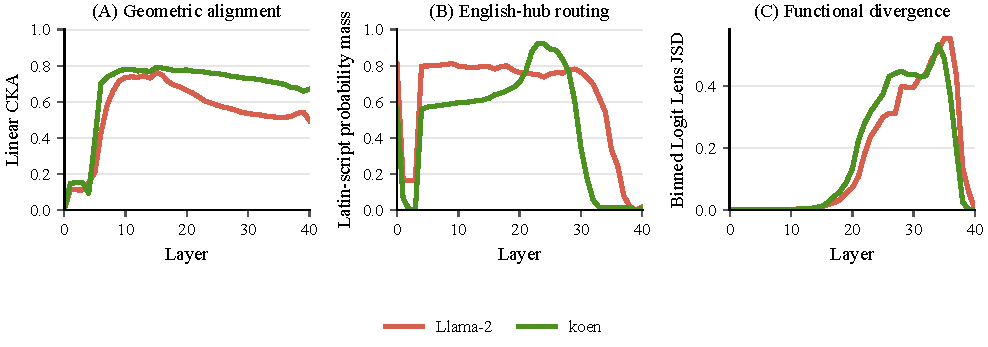
\includegraphics[width=\textwidth]{figures/fig_ko_layerwise.pdf}
  \caption{English-Korean replication, full layerwise. (A) Linear CKA between English and Korean representations. (B) English (Latin) script mass on Korean input. (C) Binned Logit Lens JSD between English and Korean predictions. The Korean-adapted koen model sustains higher CKA, reduces mid-layer English-script mass, and also shows a late-layer JSD rise.}
  \label{fig:ko_layerwise}
\end{figure*}

\subsection{Behavioral Bias Is Language-Specific}

Reading out the model's answer (context $+$ question $+$ options), every model assigns higher probability to the \emph{stereotyped} answer in English than in the translated language (Table~\ref{tab:bias}). The gap ranges from 0.13 to 0.14 across all three models, with bootstrap 95\% CIs excluding zero; the translated language sits near the three-way chance level of 0.33 while English is well above it. Translated bias benchmarks therefore do detect a real signal (English-language processing is measurably more stereotype-leaning), but the size of this cross-lingual gap is itself a property worth explaining.

\begin{table}[t]
\centering\small
\begin{tabular}{lccc}
\toprule
\textbf{Model} & $P_{\text{ster}}$(EN) & $P_{\text{ster}}$(JA) & \textbf{diff [95\% CI]} \\
\midrule
Llama-2 & 0.487 & 0.344 & 0.142 [0.094, 0.191] \\
Swallow & 0.496 & 0.352 & 0.144 [0.097, 0.192] \\
LLM-jp & 0.473 & 0.343 & 0.130 [0.078, 0.181] \\
\bottomrule
\end{tabular}
\caption{Probability of the stereotyped answer in ambiguous contexts, English vs.\ Japanese (three-way chance $=0.33$). All differences are significant (bootstrap 95\% CI excludes 0).}
\label{tab:bias}
\end{table}

The asymmetry is not uniform across stereotype types (Table~\ref{tab:category}, pooled over the three Japanese-side models). It is significant for age, disability, gender, and sexual orientation, but vanishes for physical appearance, where both languages are equally stereotype-leaning ($P_{\text{ster}}\approx0.46$). Some stereotype dimensions are thus cross-culturally shared while others are amplified in English.

\begin{table}[t]
\centering\small
\begin{tabular}{lccc}
\toprule
\textbf{Category} & $P_{\text{ster}}$(EN) & $P_{\text{ster}}$(JA) & \textbf{diff} \\
\midrule
Age & 0.491 & 0.305 & $+0.186$* \\
Disability & 0.477 & 0.305 & $+0.172$* \\
Gender identity & 0.577 & 0.446 & $+0.132$* \\
Physical appearance & 0.462 & 0.463 & $-0.001$\phantom{*} \\
Sexual orientation & 0.444 & 0.271 & $+0.173$* \\
\bottomrule
\end{tabular}
\caption{Stereotype probability by category, English vs.\ Japanese, pooled over the three Japanese-side models ($n$ from 72 to 414 per category). *: bootstrap 95\% CI excludes 0. The English-over-Japanese asymmetry holds for every category except physical appearance.}
\label{tab:category}
\end{table}

\paragraph{Korean behaves differently.} The English-over-target asymmetry does not transfer to Korean (Table~\ref{tab:ko_bias}). For the English-centric base, English is only modestly more stereotype-leaning than Korean ($+0.053$, 95\% CI $[+0.006, +0.103]$), and after Korean adaptation the gap disappears (koen: $-0.034$, CI includes 0). Crucially, where Japanese sits near chance ($\approx0.34$), Korean is nearly as stereotype-leaning as English, from $\approx0.51$ to $\approx0.54$. The cross-lingual asymmetry is therefore language-specific in magnitude, not a universal English-over-target effect; this is visible only because we measured Korean behavior directly rather than assuming the Japanese pattern.

\begin{table}[t]
\centering\scriptsize
\setlength{\tabcolsep}{2.8pt}
\begin{tabular}{@{}lccc@{}}
\toprule
\textbf{Model} & $P_{\text{ster}}$(EN) & $P_{\text{ster}}$(KO) & \textbf{diff [95\% CI]} \\
\midrule
Llama-2 & 0.562 & 0.508 & $+0.053$ [$+0.01$, $+0.10$] \\
koen & 0.507 & 0.541 & $-0.034$ [$-0.08$, $+0.01$] \\
\bottomrule
\end{tabular}
\caption{Korean behavioral bias (261 items, three-way chance $=0.33$). English is modestly more stereotype-leaning for the base model and the gap vanishes after Korean adaptation; unlike Japanese, Korean sits well above chance. Contrast with the Japanese gap of $0.13$ to $0.14$ in Table~\ref{tab:bias}.}
\label{tab:ko_bias}
\end{table}

\subsection{Hub Routing Does Not Transplant Bias}

Does the English-hub routing of \S4.2 \emph{cause} the bias of \S4.3? If a Japanese answer is computed via an English-routed representation, injecting the English state should pull the Japanese stereotype preference toward the English one. It does not. Patching the English hub-layer state into Japanese processing leaves the stereotyped minus anti-stereotyped gap statistically unchanged relative to a random-English control, in every model (Figure~\ref{fig:patch_null}). This holds both when we patch the single CKA-peak layer and when we patch the entire hub band (layers 10 to 25): the multi-layer intervention perturbs the output strongly (it shifts the gap by $-0.03$ on average) but \emph{non-specifically}: paired and random English states are indistinguishable. The English-hub representation is present, yet it does not carry the item-specific bias to the output. Korean patching gives the corresponding null result: injecting the English hub state at the CKA-peak layer into Korean processing leaves the gap unchanged versus control for both the base model and koen (transplant effect $+0.000$ and $+0.003$, 95\% CI includes 0; Figure~\ref{fig:patch_null}), so the dissociation is not Japanese-specific.

\begin{figure}[t]
  \centering
  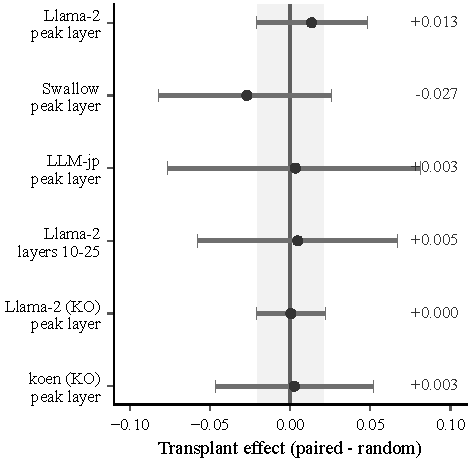
\includegraphics[width=\columnwidth]{figures/fig_patching_null.pdf}
  \caption{Hub patching does not transplant bias. Points show the control-corrected transplant effect on the stereotyped minus anti-stereotyped log-prob gap (paired-English injection minus random-English control); bars are 95\% bootstrap CIs. All CIs cross zero, including the stronger full hub-band intervention and both Korean models (bottom two rows).}
  \label{fig:patch_null}
\end{figure}

% Section break
\section{Discussion}

\subsection{CKA Is Not Enough}

Prior work infers ``language-agnostic'' middle layers from geometric measures such as CKA \citep{conneau-etal-2020-emerging, muller-etal-2021-first, chi-etal-2020-finding}. Our results show this can mislead. Swallow attains the highest CKA of any model (0.88) yet predicts English tokens for more than half of its middle-layer mass on Japanese input; Llama~2's CKA equals LLM-jp's while routing four times as much through English. Geometric alignment of a representation space does not reveal which language the model is computing in. Cross-lingual representation studies should pair CKA with a functional or script-level probe; because our models are untied, we treat the lens as suggestive and anchor the causal claim on patching.

\subsection{A Dissociation Between Representation and Behavior}

Putting the three findings together yields a dissociation. \emph{At the representation level}, a translated probe is not processed comparably: non-English inputs route through an English hub (\S4.2), to a degree set by training regime, and this is invisible to CKA. \emph{At the behavioral level}, however, the measured bias is genuinely language-specific: the stereotype asymmetry is strong in Japanese but weak in Korean (\S4.3), and injecting the English hub representation does not transplant that bias into the target language (\S4.4). The cross-lingual bias-score gap is therefore \emph{not} an English-pivot artifact; it reflects real differences in language-specific behavior, even though it is computed over internal representations that are not comparable.

This has two implications for the bias-benchmark community. A translated benchmark's per-language scores are meaningful behavioral signals, not mere echoes of English. But the internal route by which they are produced differs across languages and is hidden from geometric similarity, so \emph{representation-level} cross-lingual claims (``the model represents this bias the same way in both languages'') are not licensed by high CKA.

\subsection{Audit Protocol}\label{sec:protocol}

We distill this into a four-step protocol for translated bias benchmarks:

\begin{enumerate}
\item \textbf{Tokenizer feasibility.} Check that the tokenizer represents both languages without extreme fragmentation. Models trained from scratch on the target language only (e.g.\ Stockmark, which fragments English $\sim$34$\times$) fail here and cannot be compared cross-lingually.
\item \textbf{Geometric \emph{and} script-level convergence.} Report CKA \emph{and} a multi-anchor lens. High CKA with high foreign-script mass signals English-hub routing, so representation-level comparability claims should be withheld.
\item \textbf{Behavioral validity over representational comparability.} Treat per-language bias scores as language-specific behavior. Our patching shows they are not transplanted from English, so do not ``correct'' them toward English or dismiss a gap as an artifact by default.
\item \textbf{Surface-form fidelity filter.} When comparing scores across languages, filter low-fidelity items with a \emph{surface-form} metric such as chrF \citep{popovic2015chrf} on a back-translation, not a representation-space cosine, which would inherit the very hub-routing confound this protocol exposes.
\end{enumerate}

Step~4 is not vacuous on our own data. Back-translating each target context to English with NLLB-200 \citep{nllb2022} and scoring chrF against the source, JBBQ items are reasonably faithful (mean chrF $51.8$) while KoBBQ Simply-Transferred items are noisier ($42.3$). Restricting the Korean comparison to above-median-fidelity items shrinks the base model's English/Korean gap from $+0.053$ to $+0.017$: a surface-form filter materially changes the measured asymmetry, exactly the items a representation-space cosine would fail to flag.

% Section break
\section{Conclusion}

Using architecture-matched models and two continual-adaptation pairs, we show that high cross-lingual CKA can hide an English-processing hub: non-English inputs are routed through English-script predictions in middle layers, to a degree that target-language adaptation reduces (Llama~2$\to$Swallow, replicated for Korean via koen) and balanced training minimizes. Yet this hub does not transplant bias: English is more stereotype-leaning, strongly in Japanese and weakly in Korean, but injecting English hub states, even across the whole hub band, does not move the target-language stereotype preference. Translated bias scores are thus genuine language-specific behavior produced over non-comparable representations, a dissociation between representation and behavior that we turn into a four-step audit protocol.

% Section break
\section*{Limitations}

\paragraph{Korean replication scale.} The English/Korean analysis uses the 261-item Simply-Transferred subset of KoBBQ and a single adapted model (koen) with a smaller adaptation corpus than Swallow; we therefore report it as a directional replication, not an equal-scale result.

\paragraph{Null result.} The patching finding is a null. We strengthen it by testing both the CKA-peak layer and the full hub band and by showing the multi-layer patch does perturb outputs (so the null is not a dead intervention), but a null cannot establish the strict absence of any bias transplant.

\paragraph{Untied embeddings.} All models have untied embeddings, which weakens the raw Logit Lens; we mitigate by keeping the condition uniform across models and anchoring causal claims on patching rather than the lens.

\paragraph{Tokenizer is part of the regime.} The matched pairs differ in vocabulary (Swallow and koen extend Llama~2's tokenizer), so ``adaptation'' bundles continual pretraining with tokenizer extension; we do not separate the two.

\paragraph{Scope.} Three training regimes, two target languages (both adapted from the same English base), 2023-era 13B base models, and template-based probes. Instruction-tuned models, other language families, and naturalistic probes remain future work.

\section*{Ethical Considerations}

This work studies stereotype bias in order to improve how cross-lingual bias benchmarks are interpreted, not to build or amplify biased systems. It uses existing public benchmarks (BBQ, JBBQ, KoBBQ) and open-weight models, and collects no new human-subject data. Our findings are specific to the models, languages, and template-based probes studied; in particular, we find that the studied models are measurably more stereotype-leaning in English than in Japanese, so the results should not be read as certifying any model as unbiased. The audit protocol aims to make cross-lingual bias measurement more trustworthy, but passing it does not certify a model as fair.

\balance
\bibliography{main}

\clearpage
\appendix

\section{Implementation Details}
\label{app:implementation}

\paragraph{Answer scoring.} For each ambiguous item, we concatenate the prompt with each of the three answer options and score only the candidate tokens:
\[
s(a)=\sum_{j=1}^{|a|}\log p(a_j \mid \text{prompt}, a_{<j}).
\]
We report the stereotyped minus anti-stereotyped gap $s(a_{\text{ster}})-s(a_{\text{anti}})$ for patching and convert the three option scores to $P_{\text{ster}}$ by a softmax over \{stereotyped, anti-stereotyped, unknown\}. The same scoring rule is used for English, Japanese, and Korean.

\paragraph{Semantic-bin lens.} The binned Logit Lens uses fixed bilingual lexical anchor sets covering age, gender, ability/disability, valence, hierarchy, and trait terms. For each bin, we tokenize every anchor with the model tokenizer, sum the layerwise probability assigned to the resulting token ids, and renormalize over bins before computing JSD. This probe is intentionally coarse: it is used to check whether high CKA coexists with functional divergence, not to define a task-level semantic parser.

\paragraph{Patching.} For a patch layer $\ell$, we run the English prompt, store the final-prompt-token hidden state at layer $\ell$, and during target-language candidate scoring replace the corresponding final-prompt-token block output with that vector. The single-layer intervention uses the CKA-peak layer; the stronger intervention patches every layer in the hub band 10 to 25. The random control uses English states from a different item with the same layer set, so the reported transplant effect is paired-English injection minus random-English injection.

\paragraph{Surface-form fidelity.} We back-translate target contexts to English with NLLB-200 and score chrF against the English source. We use chrF rather than embedding cosine because representation similarity can reflect English-hub routing. KoBBQ-aligned chrF then supports the median filter in \S\ref{sec:protocol}.

\section{Supplementary Layerwise Figures}
\label{app:figures}

\paragraph{Binned Logit Lens JSD.} Figure~\ref{fig:jsd} plots the binned Logit Lens Jensen-Shannon divergence between English and Japanese predictions at each layer. For Llama~2 and Swallow it is near zero through the middle layers and rises to a late-layer peak (0.55 and 0.59 at layers 36 and 35), where each language resolves to its own surface forms; the balanced LLM-jp stays near zero throughout. Functional divergence therefore emerges despite the high mid-layer CKA reported in the main text.

\begin{figure}[H]
  \centering
  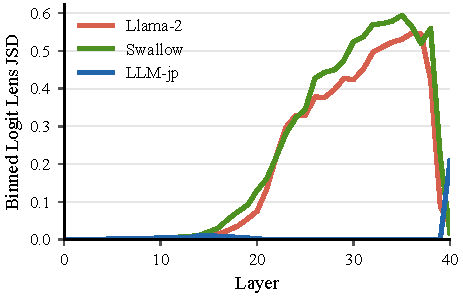
\includegraphics[width=\columnwidth]{figures/fig_jsd_layerwise.pdf}
  \caption{Binned Logit Lens JSD between English and Japanese predictions, per layer. Near zero through the middle layers (functional convergence), peaking late as each language resolves to its own tokens; LLM-jp diverges least.}
  \label{fig:jsd}
\end{figure}

\paragraph{Interpreting late-layer divergence.} The late JSD rise should not be read as contradicting the mid-layer hub result. It appears after the hub band, when the model resolves to language-specific surface forms, whereas the main comparability question concerns the middle layers where CKA is high and script routing differs. We therefore use the binned lens as a corroborating functional probe and rely on patching, rather than the untied Logit Lens alone, for the causal claim.

\end{document}
